\section{Constraints}
constraints in design and implementation

\subsection{Riot API Ratelimits}\label{riot-api-ratelimits}
Für die API von Riot Games gibt es zwei verschiendene API Keys. Den Development Key und den Production Key. Einen Development Key kann hier jeder beantragen, für einen Production Key hingegen muss ein bereits fertiges Produkt vorhanden sein, welches dann noch durch einen Application Prozess angenommen werden muss.\\
Ein Production Key sind 500 Request alle 10 Sekunden bzw. 30.000 Requests alle 10 Minuten erlaubt.\\
Für dieses Projekt wird ein Development Key verwendet. Für diesen sind die Ratelimits deutlich geringer, mit 20 Requests pro Sekunde bzw. 100 Requests alle 2 Minuten.\\
Für die Demonstration dieses Projekts sind aber auch diese deutlich geringeren Ratelimits ausreichend, da nie mehr als 1-2 Leute gleichzeitig auf die Website zugreifen und die Anzahl der gespeicherten Spieler gering bleibt.\\
Möchte man die Website später öffentlich zugänglich machen, so müsste ein Production Key verwendet werden, da Riot es nicht erlaubt Development Keys für öffentliche Produkte zu verwenden und die Ratelimits nicht ausreichend währen.

\subsection{Server Performance}

Als Infrastruktur wurde der Landesdienst von bwCloud verwendet, der eine kostenlose
"Infrastructure-as-a-Service" Umgebung für Forschung und Lehre in Baden-Württemberg bereitstellt.
Wie Grafik \ref{fig:uebersicht_kontingente} zeigt, kann pro Nutzer nur ein bestimmtes Kontingent an VCPUS, RAM sowie Datenträger-Speicher verwendet werden.
Sobald mehr Server-Ressourcen benötigt werden, ist dies nicht möglich ohne auf einen kostenpflichtigen Dienst wechseln zu müssen.

\begin{figure}
\centering
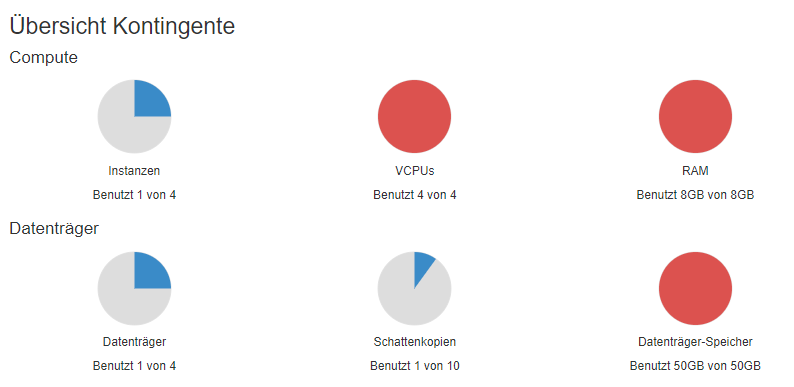
\includegraphics[width=0.8\textwidth]{uebersicht_kontingente.png}
\caption{Übersicht der verfügbaren Kontigente}
\label{fig:uebersicht_kontingente}
\end{figure}

Diese beschränkten Ressourcen haben einen direkten Einfluss auf die Ausführung von komplexen Datenbankoperationen. Außerdem ist ein
horizontales Scaling des Dienstes durch die Limitierung ebenso nicht möglich, wodurch nur die Performance durch verbesserte SQL-Abfragen
optimiert werden kann.
